%%=============================================================================
%% Methodologie
%%=============================================================================

\chapter{Testopstelling}
\label{ch:testopstelling}
 
Om dit alles te testen werd er gebruik gemaakt van een Cisco 2960 Series switch die geproduceerd is in 2006. Het model van deze is meer bepaald de C2960-24LT die een 24 100Mbit poorten heeft waarvan er acht voorzien zijn van POE. Als laatste zijn er nog twee Gigabit interfaces aanwezig. De switch had versie 12.2(44R)SE1 geïnstalleerd bij het uitvoeren van de tests.
Deze kwam nieuw uit de doos dus stond deze bij het ontvangen volledig op standaardinstellingen. Hierna werd er gekeken hoe we de werkelijkheid zoveel mogelijk konden nabootsen. Daarom is de switch tijdens het configureren over SSH achter een router geplaatst. Op deze manier was het bijvoorbeeld ook heel eenvoudig om via een laptop op afstand en over een WiFi-netwerk het apparaat te beheren, ongeveer zoals dit in werkelijkheid zou verlopen.
\\

Omdat er voor het instellen van de basisconfiguratie nog nood is aan een console connectie werd een seriële kabel met usb aansluiting aangekocht, dit is goedkoop terug te vinden op Ebay en werk met nieuwere computers prettig en hiervoor was ook geen installatie nodig. Dit was noodzakelijk omdat veel computers tegenwoordig geen DB9 aansluiting meer hebben, hoewel dit de enige kabel is die meegeleverd wordt met een Cisco switch.

\begin{figure}[H]
\centering
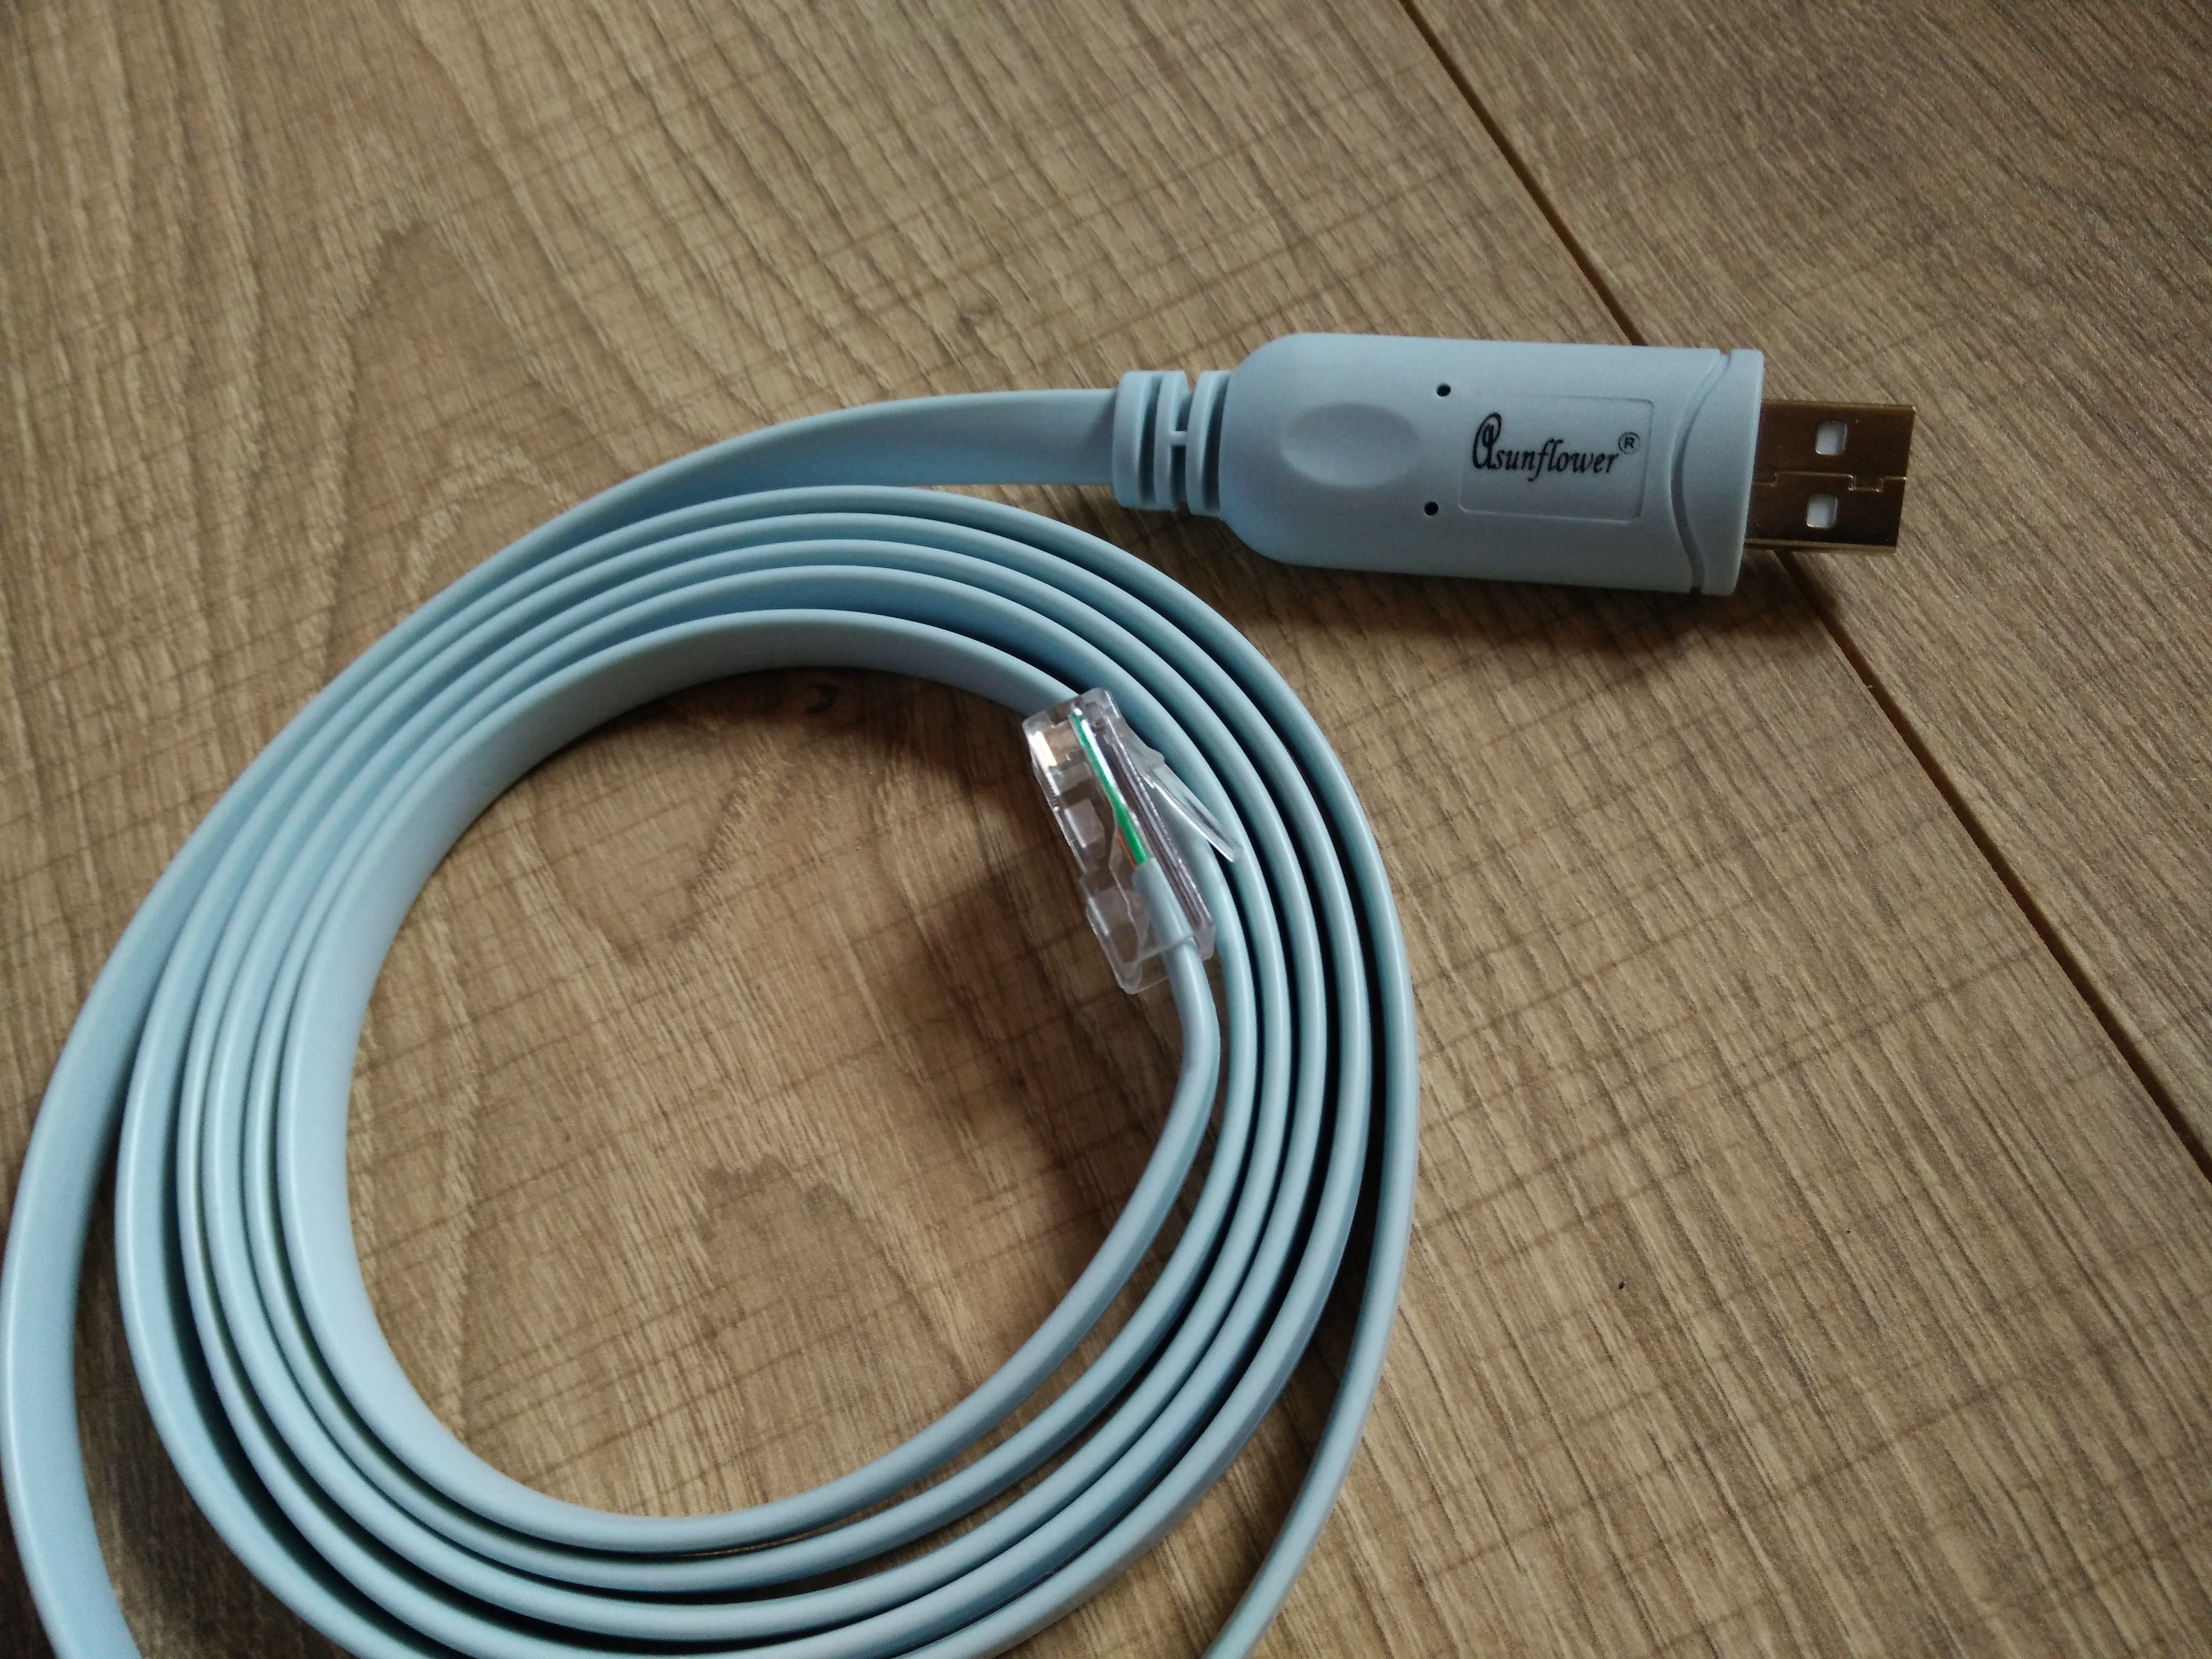
\includegraphics[width=10cm]{../img/serialcable}
\caption{De aangekochte seriële consolekabel, deze is te vinden op Ebay als een 'FTDI USB to RJ45'. Er wordt ook duidelijk vermeld dat dit specifiek voor Cisco apparaten is. }
\end{figure}

Om deze in gebruik te nemen bij Windows is het even kijken onder apparaatbeheer welke poort deze precies in beslag neemt. Dit kan je terug vinden onder de sectie 'poorten'. Op mijn apparaat was dit COM4. Hierna kan je in Putty bij seriële connectie gewoon COM1 aanpassen naar COM4 en de juiste snelheid meegeven, dit staat standaard correct maar indien dit niet zo is moet het 9600 zijn. Daarna kan je aan de slag met het apparaat zoals gewoonlijk.
\\

Op een Apple computer is de procedure een klein beetje anders. Het is een beetje zoeken hoe het apparaat precies noemt maar via tabcompletion is het vrij eenvoudig terug te vinden.
\begin{center}
\begin{BVerbatim}
$ screen /dev/tty.usb
	% invoer van tab
$ screen /dev/tty.usbserial-AK05D1K3
switch1>
\end{BVerbatim}
\end{center}

Verder is het noodzakelijk om op de switch een ip adres in te stellen en een default gateway. Enkel op deze manier is het mogelijk om een connectie vanop afstand te maken met de switch. Verder om een SSH verbinding tot stand te kunnen brengen is er een username en een wachtwoord nodig, ook dit moet ingesteld worden. Als laatste wordt een SSH key aangemaakt. Vanaf dan is het mogelijk om via SSH connectie te maken, zoals je met een server zou doen. Dit kan via Putty op Windows of via het SSH commando op bijna ieder unix systeem. Dit is hoe Ansible en NAPALM connectie zullen maken met het apparaat dus deze stap is cruciaal voor het verdere proces.
\begin{figure}[H]
\centering
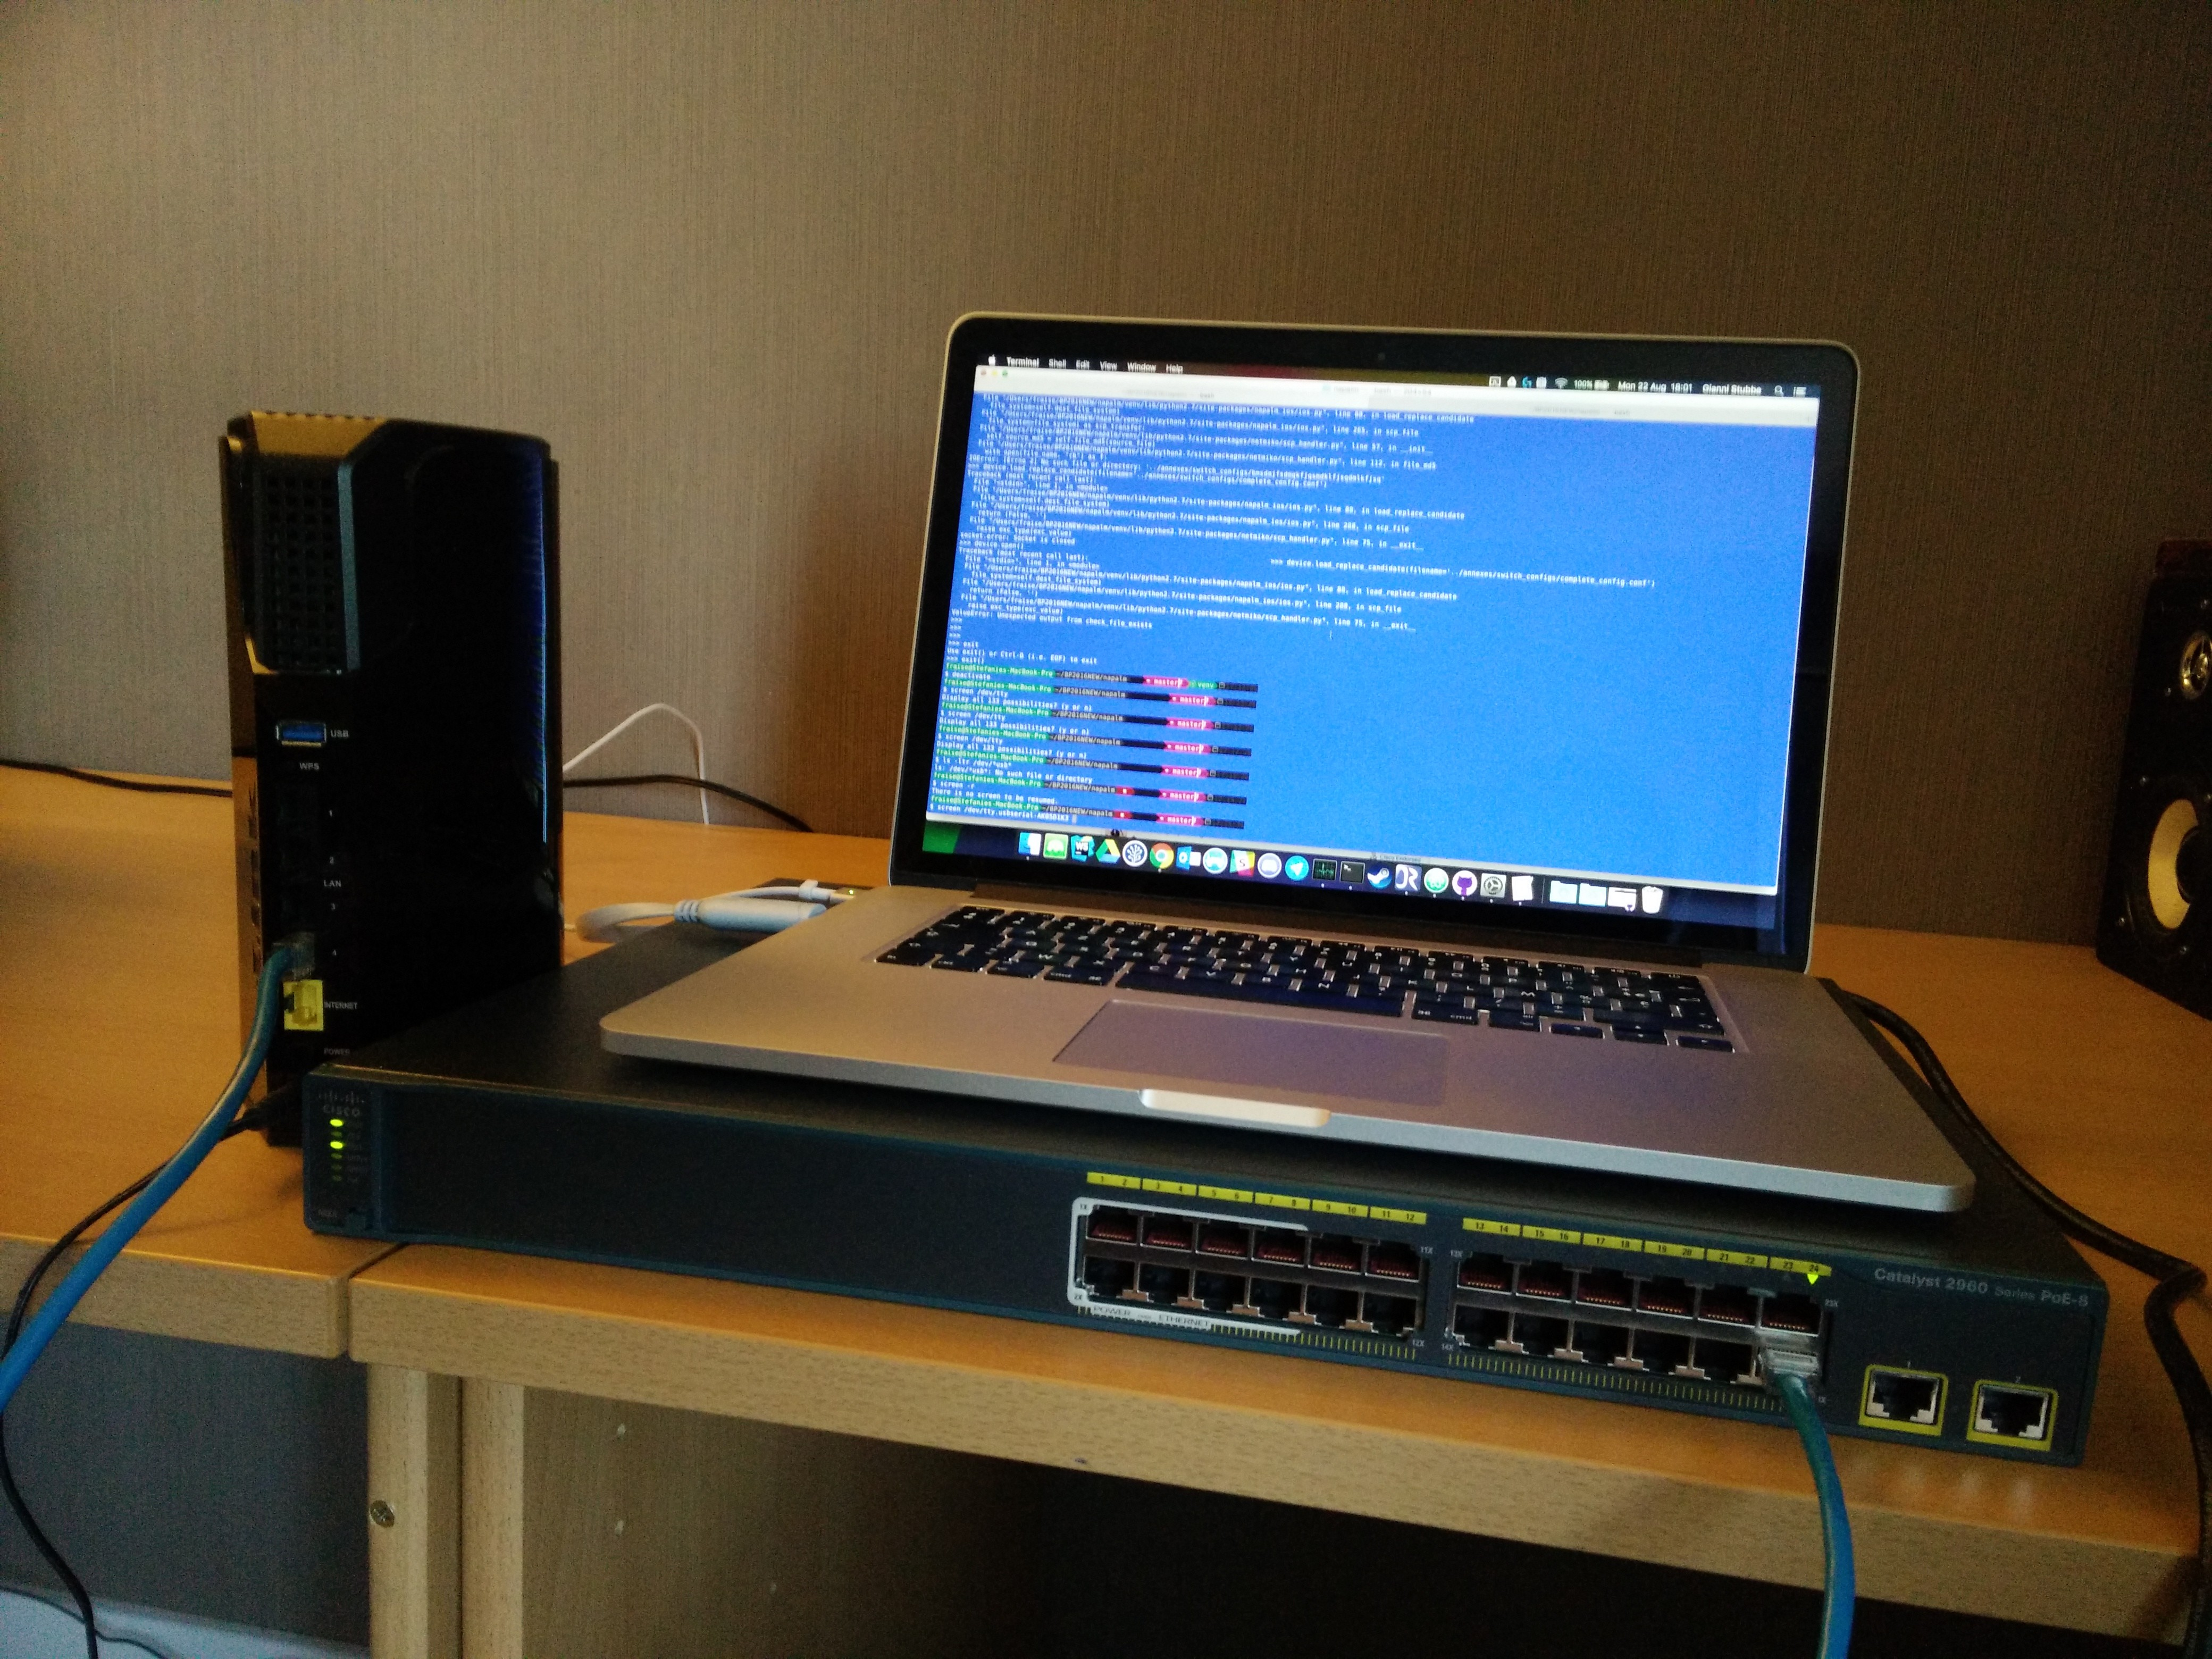
\includegraphics[width=15cm]{../img/setup}
\caption{Links op de afbeelding de router met ip adres: 172.17.1.1 deze is aangesloten op de switch poort fa0/24. Deze behoort tot vlan1 die het ip adres 172.17.1.2 heeft. Daarboven een laptop die via usb console kabel aan de switch verbonden is en via wifi aan de router. Op deze manier was het eenvoudig de switch resetten via console kabel en eenvoudig Ansible uit te voeren over WiFi dan. }
\end{figure}

Na het opstellen van deze testopstelling werd er over gegaan op het configureren van de switch met de basis instellingen die benodigd zijn voor SSH connecties toe te staan.




